\section{Métodos}

Se estudió un circuito RC de distribución desconocida (\autoref{fig:arreglo}) con el objetivo de modelar su composición en función de su comportamiento a distintas señales, para ello se realizaron diferentes experimentos. Un experimento consisitió en variar la frecuencia de la señal sinusoidal de entrada, dada por un generador de ondas $Sinometer$ modelo VC2002 \cite{VC2002} o un generador de ondas $OWON$ modelo DG31000 \cite{DGE1000}, manteniendo la amplitud constante y variando la frecuencia $f$ en el rango [0,01; 60] \SI{}{\kilo\hertz}. La señal de entrada $V_{in}$ y la señal de salida $V_{out}$, se registraron simultáneamente utilizando un osciloscopio $Tektronix$ modelo TDS 220 \cite{TDS200}. A partir de estos datos se calculó la impedancia del sistema como el cociente entre las amplitudes de entrada y salida. Además, en cada medición se registró la diferencia temporal $\Delta t$ entre ellas. A partir de estos datos se calculó el respectivo desfasaje mediante la relación $\varphi=2\pi f \Delta t$, donde $f$ es la frecuencia de $V_{in}$ y $\omega=2\pi f$. Se realizaron entonces diagramas de Bode mediante el gráfico del módulo de la impedancia y la fase a fin de obtener información sobre la composición del circuito. También se construyeron diagramas de Nyquist, ya que representan gráficamente la respuesta del sistema según su geometría, a partir de  la parte imaginaria de la impedancia en función de su parte real. A partir de estos gráficos fue posible modelar el circuito y aproximar los valores de los distintos elementos que lo componen.

\begin{figure} [H]
    \centering
    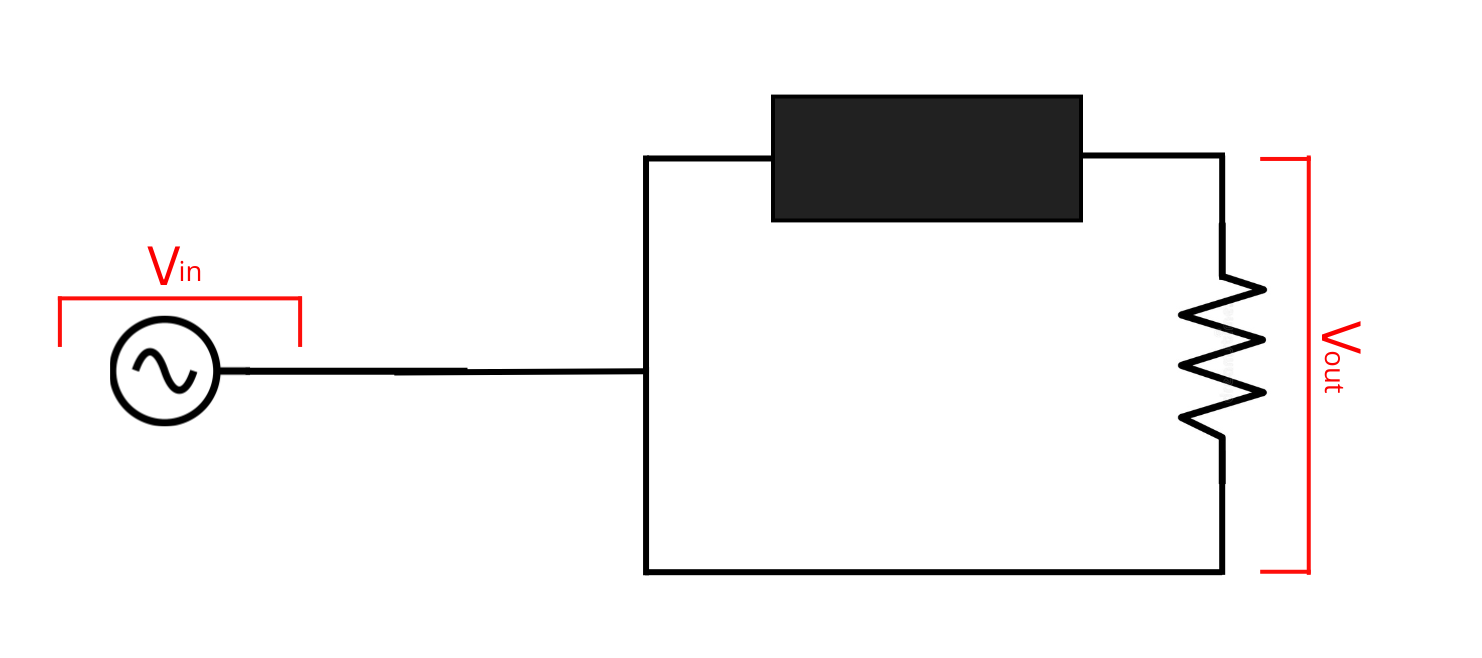
\includegraphics[width=0.6\linewidth]{Figuras/esquema.png}
    \caption{Arreglo experimental utilizado para estudiar el circuito RC de distribución desconocida. La señal de entrada $V_{in}$ y la señal de salida $V_{out}$ se midieron simultáneamente utilizando un osciloscopio.}
    \label{fig:arreglo}
    
\end{figure}

Otra de las experiencias consitió en aplicar una señal de entrada cuadrada, con el objetivo de estudiar la carga de los posibles capacitores que componen el circuito. Para ello se utilizó un generador de ondas $Sinometer$ modelo VC2002 \cite{VC2002} y un osciloscopio $OWON$ modelo VDS3104 \cite{VDS3104}. Se registró la señal de entrada y de salida, para determinadas frecuencias dentro del rango ya barrido en el experimento anterior y se estudió el comportamiento de la señal de salida en función del tiempo. A partir de estos datos se calcularon las constantes de tiempo $\tau$ que caracterizan la carga de los capacitores que componen el circuito. Por cada frecuencia, se registraron tres series que contengan al menos 6 pulsos que fueron ajustados según la ecuación \eqref{ajustepulsoscuadrados}, donde $i$ indica el número de pulso que se muestra en la pantalla. 

\begin{equation}
    V(t) = C_i + A_i e^{-t/\tau}
    \label{ajustepulsoscuadrados}
\end{equation}
